\section{Introduzione e descrizione dell'apparato sperimentale}
Per condurre l'esperienza ci siamo serviti di una Breadboard dotata di due boccole e di una griglia di fori in cui inserire i refori. La griglia è caratterizzata dalla presenza di quattro colonne indicate con i simboli "+" e "-", ciascuna equipotenziale, e altre venti colonne equipotenziali riga per riga, indicate con delle lettere. Lo strumento ci ha permesso di realizzare i circuiti su cui abbiamo condotto le diverse misure. Le componenti di circuito di cui ci siamo serviti sono state le resistenze, di cui abbiamo ricavato i valori tramite un \textit{tool online}\footnote{ https://www.digikey.it/it/resources/conversion-calculators/conversion-calculator-resistor-color-code}, diodi di silicio e un partitore resistivo, composto da boccole e da interruttori in grado di modificare la resistenza dello strumento.
Abbiamo fatto uso di due multimetri, strumenti in grado di misurare diverse grandezze, nel nostro caso utilizzati per determinare la differenza di potenziale tra due punti del circuito e l'intensità di corrente.
Infine, abbiamo collegato un generatore che fornisse corrente ai circuiti, attraverso il controllo della sua differenza di potenziale.

\begin{figure}[h!]
    \centering
    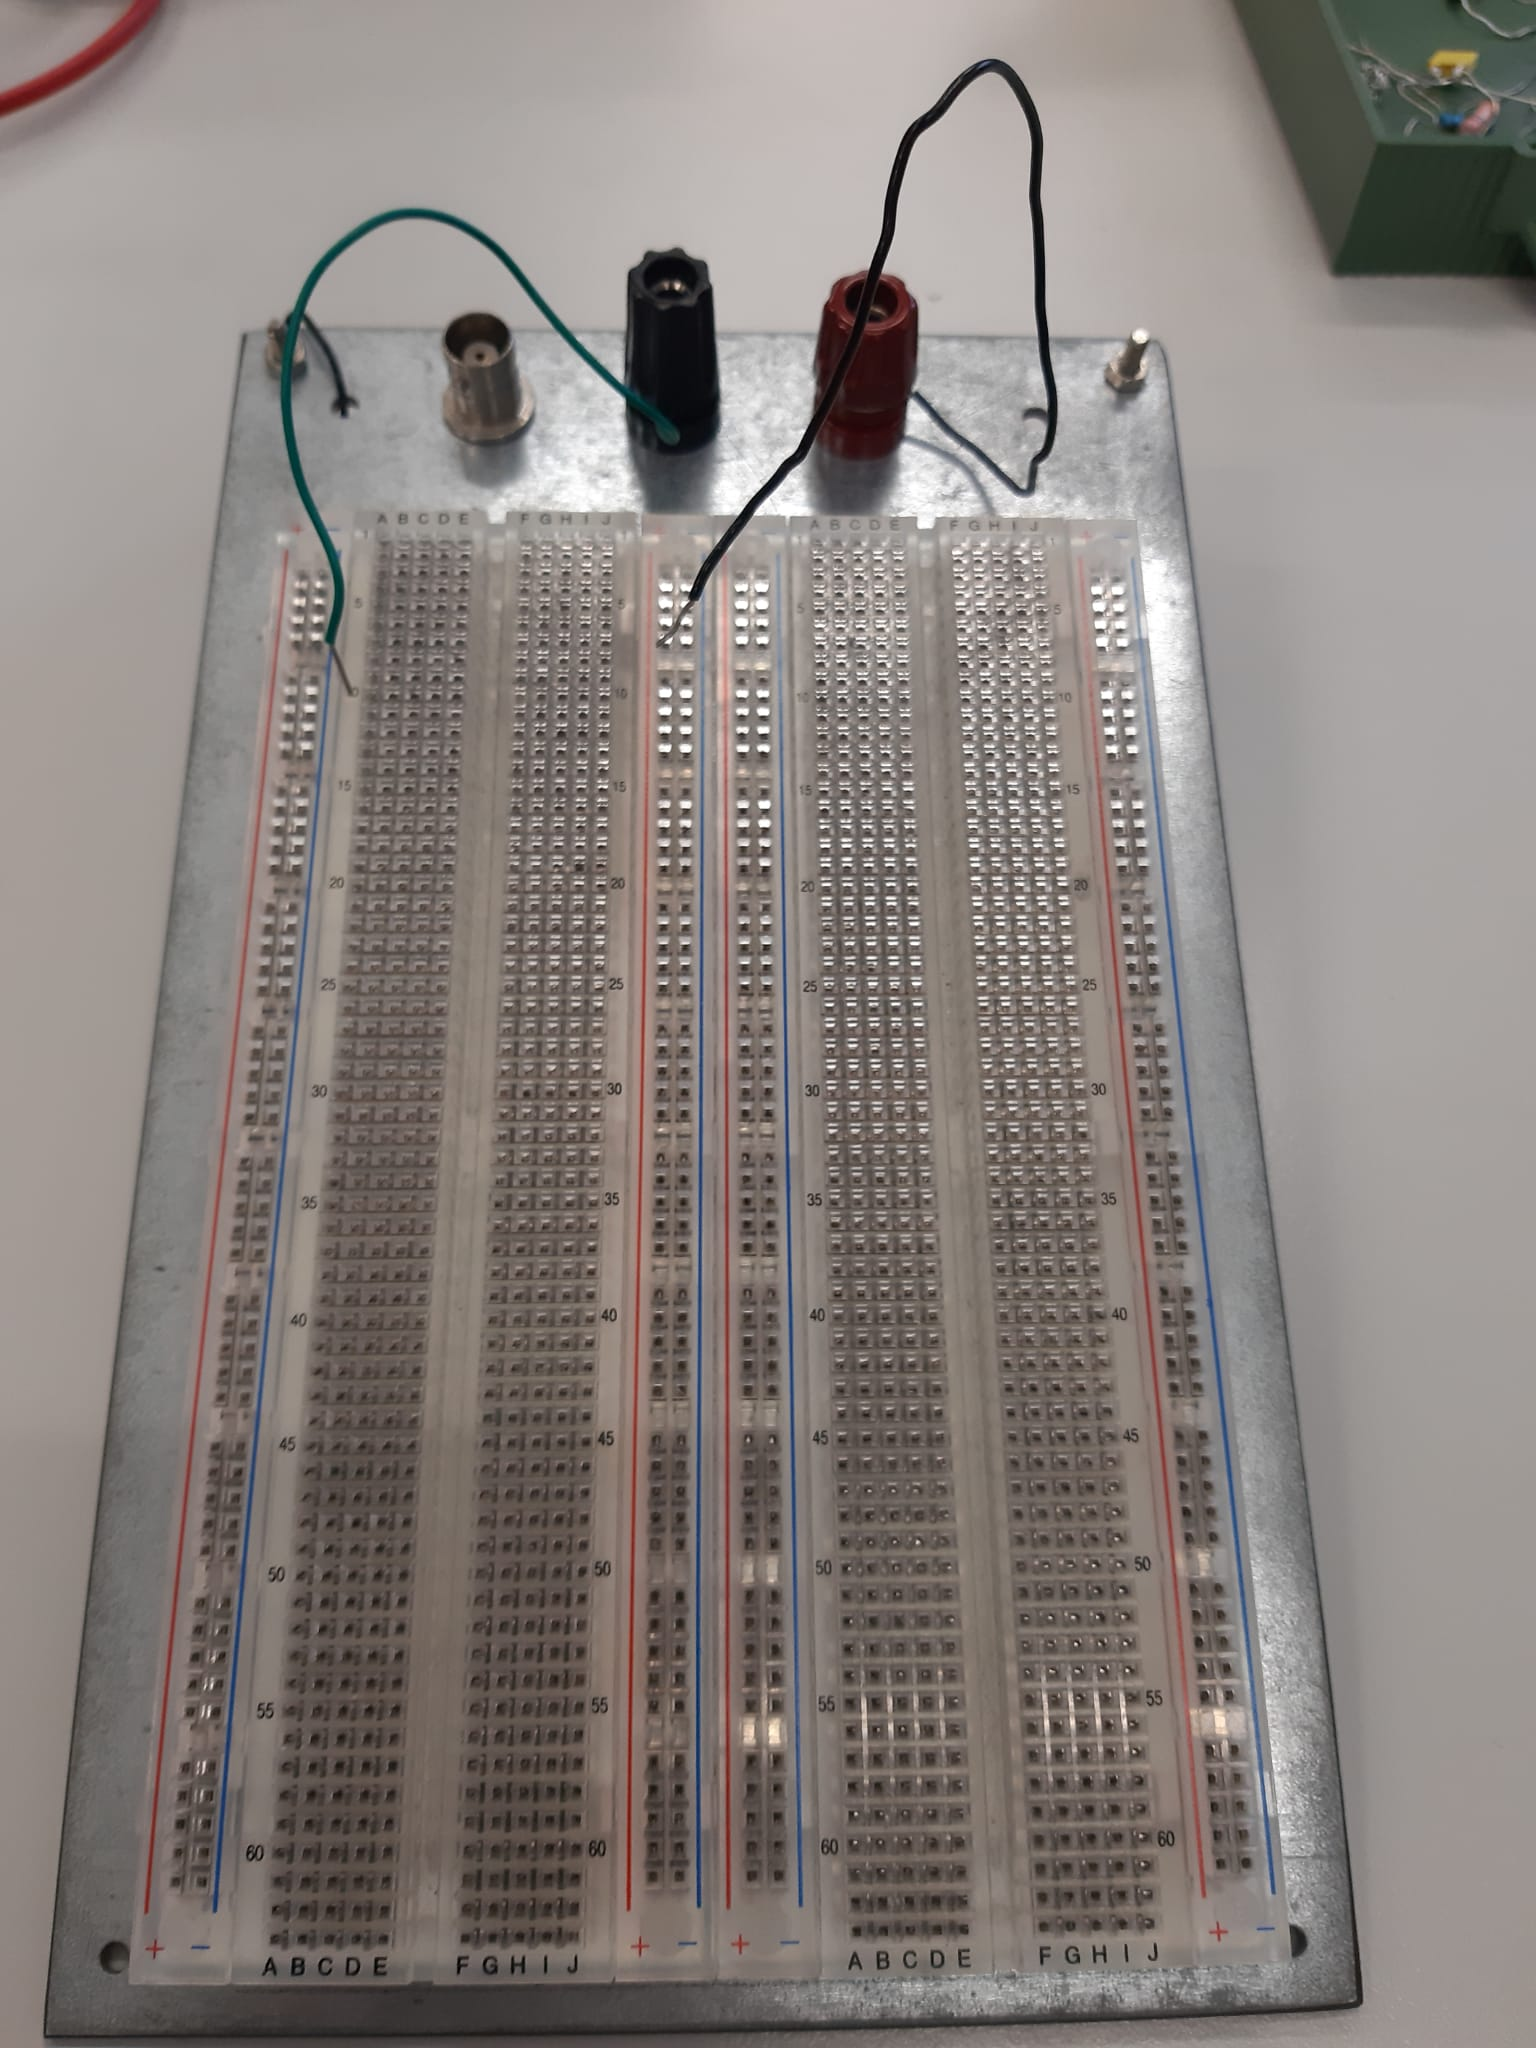
\includegraphics[scale=0.1]{Immagini/Circuitoooo.jpeg}
    \label{fig:my_label}
\end{figure}

La prima parte dell'esperienza si è concentrata sullo studio della strumentazione di laboratorio, studio finalizzato ad utilizzare configurazioni adeguate nelle parti successive. E' stato, infatti, necessario verificare che il multimetro usato come Voltmetro fosse ben progettato, cioè che avesse la caratteristica di possedere una resistenza in parallelo grande. Analogamente, è stato necessario verificare che il multimetro usato come Amperometro avesse la caratteristica di possedere una resistenza in serie piccola.
Successiavmente ci siamo concenrati sullo studio delle resistenze e della Legge di Ohm:

\begin{equation}
\frac{1}{R_{\parallel}}=\sum_{i=1}^{N}\frac{1}{R_{i}} \hspace{73 pt} R_{\perp}=\sum_{i=1}^{N}R_{i}
\end{equation}

\begin{equation}
V=R_{tot}I
\end{equation}

Infine, abbiamo studiato la Legge di Shockley, che descrive l'andamento di corrente per i diodi:

\begin{equation}
I=I_{0}(e^{qv/gK_b T}-1)
\end{equation}

indicando con \textit{q} la carica degli elettroni, con $K_b$ la costante di Boltzmann, con \textit{g} la costante che dipende dal tipo di diodo e con T la temperatura del diodo in Kelvin, corrispondente a quella dell'ambiente. Il termine di proporzionalità $I_0$ è detto \textit{intensità di corrente di saturazione}, il valore che ci aspettiamo di ottenere è molto piccolo in quanto si tratta di una corrente generata dai portatori di carica interni al diodo in diffusione dalla regione neutra alla regione di carica spaziale\footnote{Si tratta di una regione isolante all'interno di un semiconduttore drogato.}.